\todo{There should be a link either here or at end of literature which forms the basic for different methods (clustering, routing, trip generation).}
\todo{Paragraph describing different types of algorithm used (Routing then cluster, Cluster then Routing, Genetic, etc.)}
\todo{Remember to justify the choice of algorithms. You may also need to explain how to adopt these algorithms in your work. A figure showing the ralationship between different components of your work may also help.}


\subsection{Clustering}\label{subsec:clustering}
Clustering as a concept can be described as `the unsupervised classification of patterns (observation, data items, or
feature vectors) into groups (clusters)'\todo{cite Data Clustering: A review, A.K. Jain}.
In our problem, clustering will be used to group locations together to form an itinerary for each day of the trip.
These clusters (or days) will then be used as an input for some routing algorithm, which will try and find an
optimal route for each day.
These routes can then be combined to form a complete route for the trip, which can be evaluated using our cost
function.
The goal of our clustering algorithms is to find a set of clusters that, when combined with some routing algorithm,
will produce a route that minimises the cost function.\\
\\
The clustering algorithms implemented in this project are: K-Means, Genetic Clustering and Genetic Centroid-based
Clustering.

\subsubsection{K-Means}\label{subsubsec:k-means}
K-Means is an iterative clustering algorithm that defines its clusters using a set of centroids (means) which are
given a location in the input space.
The algorithm starts by initialising random centroids and iteratively improving the clustering from there, continuing
until the algorithm converges (on a local optimum) or an iteration limit is reached.
While this algorithm may not find the best solution, it is rather quick, with a time complexity of $O(kni)$, where $k$
is the number of clusters, $n$ is the number of locations and $i$ is the maximum allowed number of iterations.\\

\noindent
In our implementation of K-Means we will initialise our centroids by generating random geographic coordinates in
a similar area to the locations in our input.
We will be using the coordinates of our locations to calculate the Euclidean distances between locations and centroids,
these locations will be assigned to the cluster of the closest centroid.

\begin{figure}[H]\label{fig:_assign_nodes_to_centroid}
    \centering
    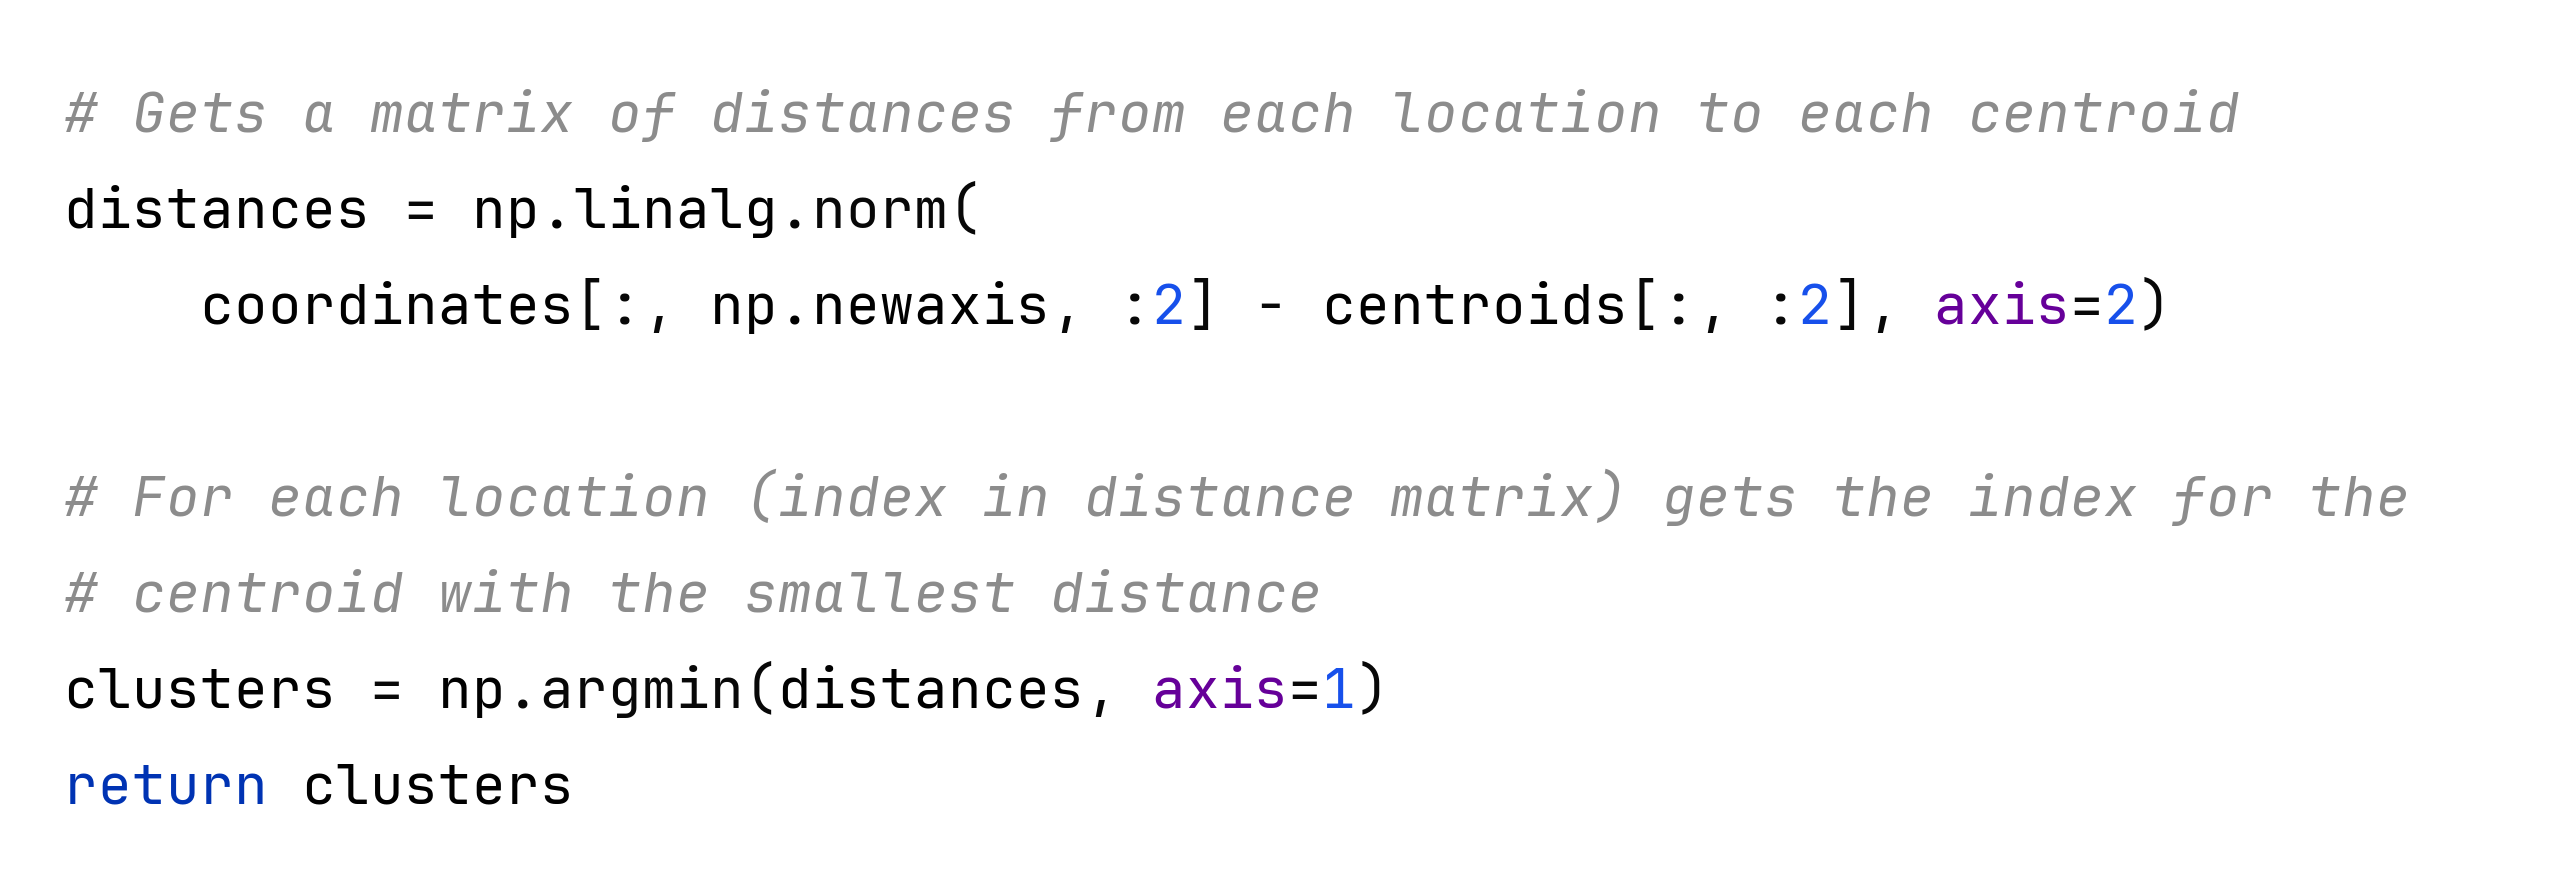
\includegraphics[width = \textwidth]{Clustering._assign_nodes_to_centroid}
    \caption{Clustering.\_assign\_nodes\_to\_centroid in algorithms\textbackslash clustering.py}
\end{figure}
\noindent
After assignment, the centroids are recalculated such that their coordinates are the average of all locations
assigned to their cluster.

\begin{figure}[H]\label{fig:_compute_means}
    \centering
    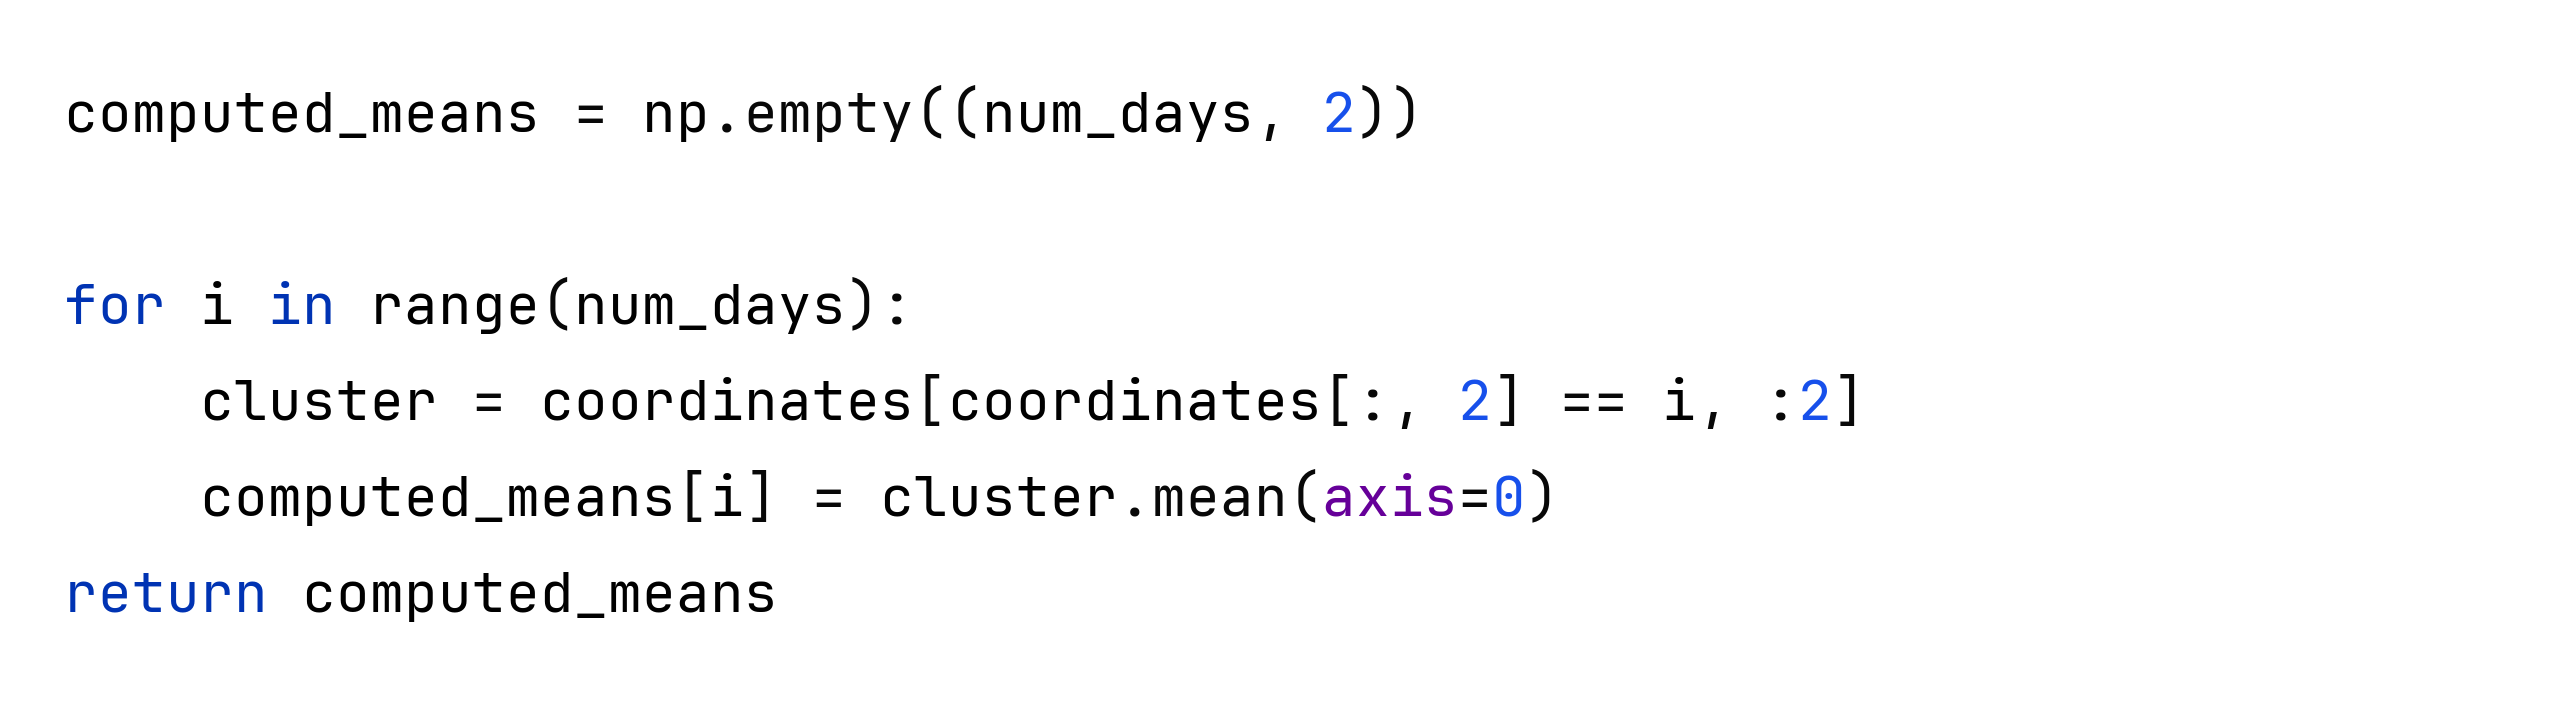
\includegraphics[width = \textwidth]{KMeans._compute_means}
    \caption{KMeans.\_compute\_means in algorithms\textbackslash clustering.py}
\end{figure}
\noindent
These steps of cluster assignment and centroid recalculation are repeated until either a maximum allowed number of
iterations is reached, or until the algorithm converges on an optimum solution.
Our convergence criterion is that the centroids stop changing between iterations, i.e., the centroids are the same
as the previous iteration.

\begin{figure}[H]\label{fig:find_clusters}
    \centering
    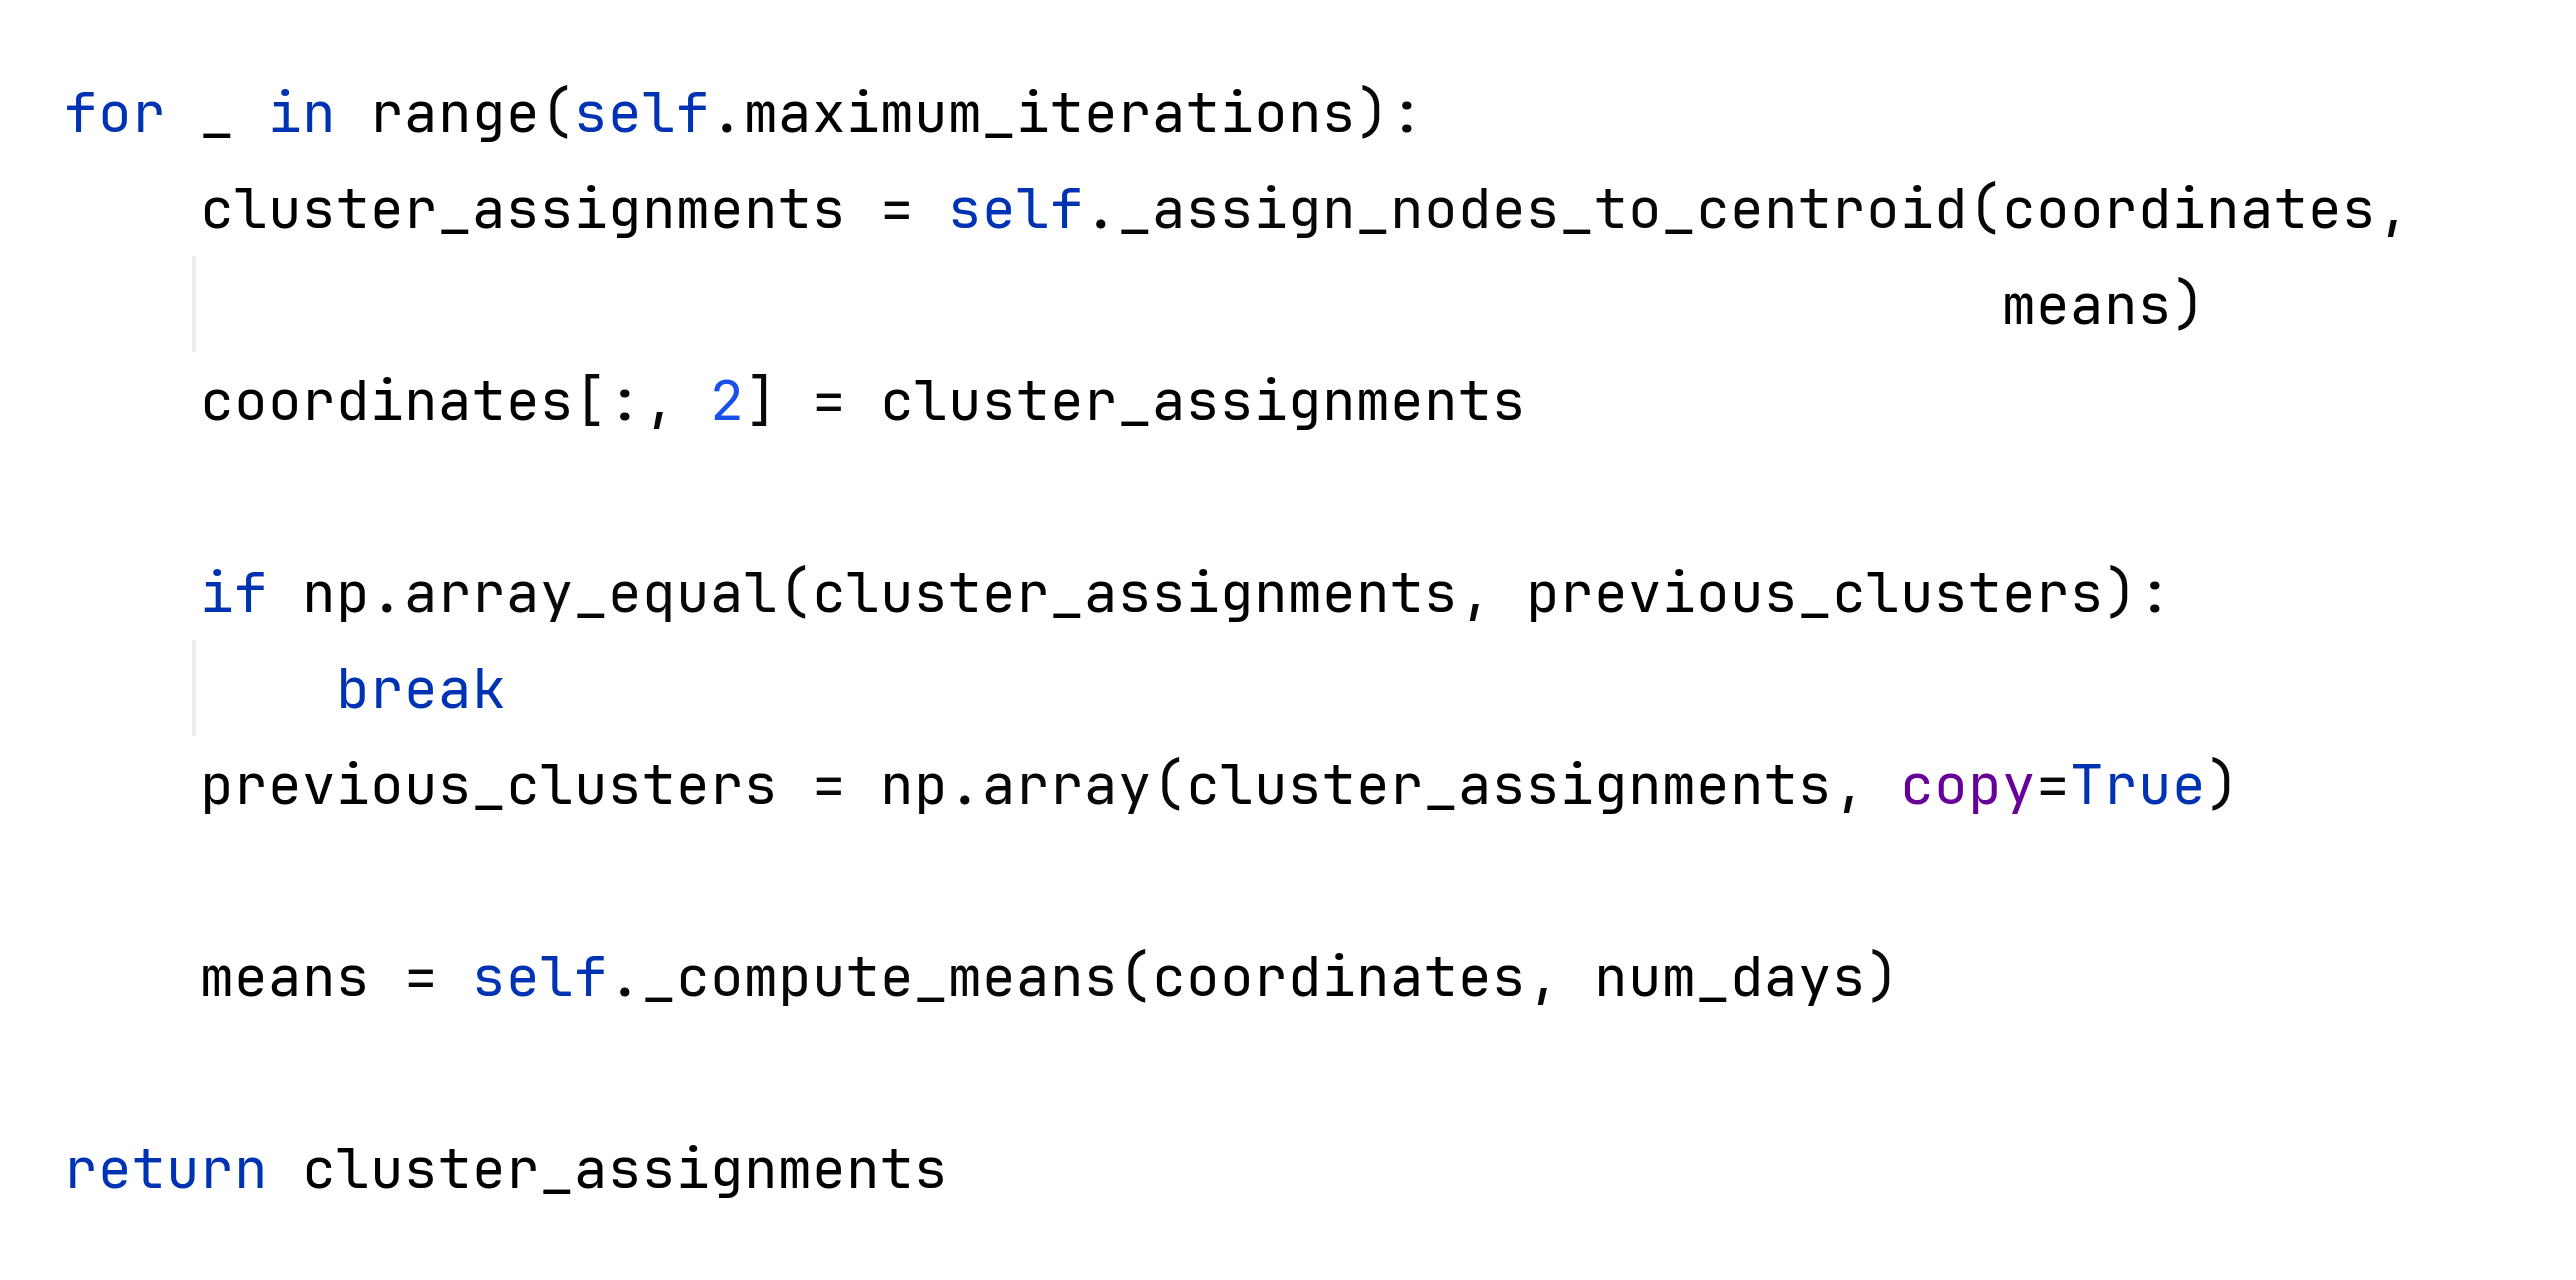
\includegraphics[width = \textwidth]{KMeans.find_clusters}
    \caption{KMeans.find\_clusters in algorithms\textbackslash clustering.py}
\end{figure}
\\
\noindent
Below is an example of the K-Means algorithm run on an input of 25 points of interest around London over seven days.

\begin{figure}[H]
    \ContinuedFloat*
    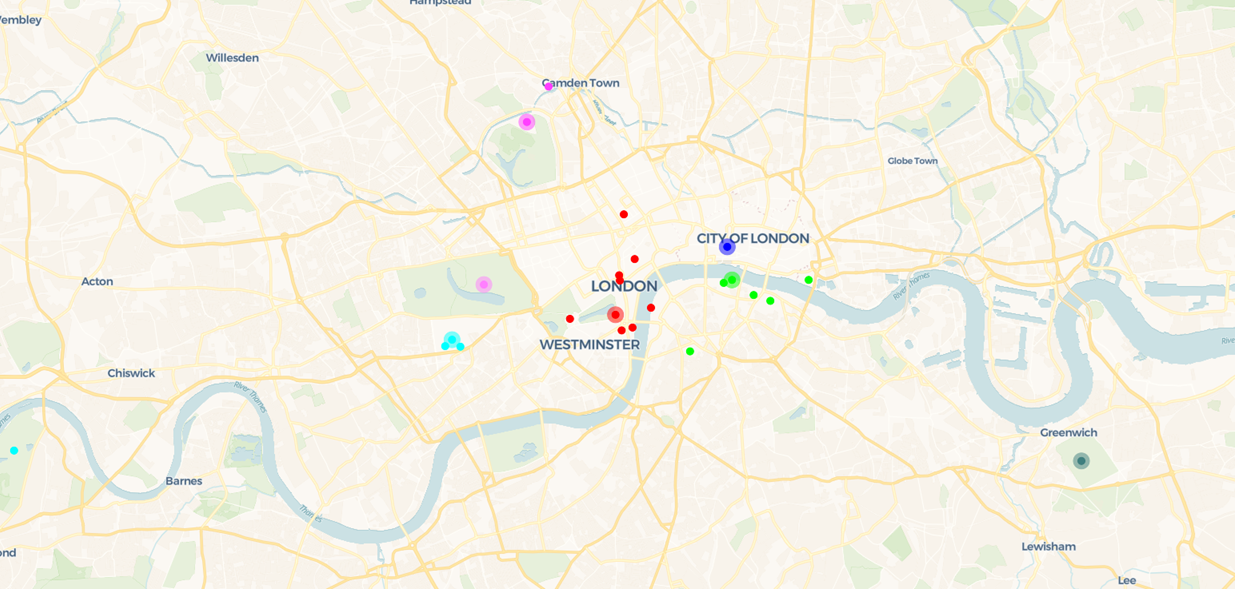
\includegraphics[width = \textwidth]{KMeans_London_Step1}
    \caption{Step1}
\end{figure}
\begin{figure}[H]
    \ContinuedFloat
    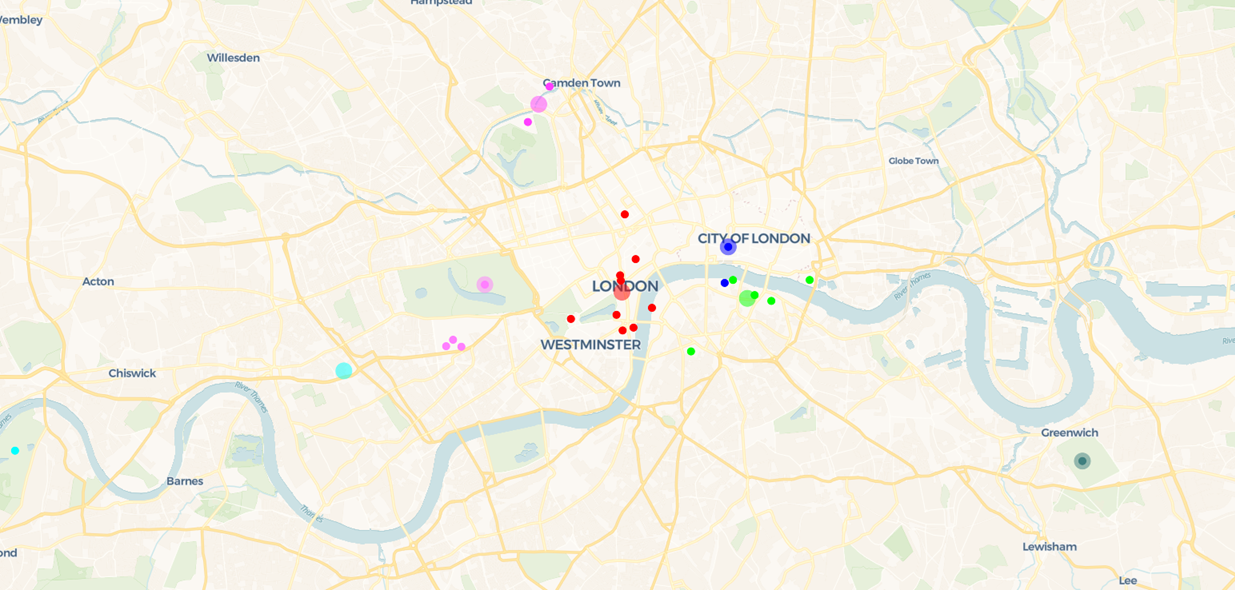
\includegraphics[width = \textwidth]{KMeans_London_Step2}
    \caption{Step2}
\end{figure}
\begin{figure}[H]
    \ContinuedFloat
    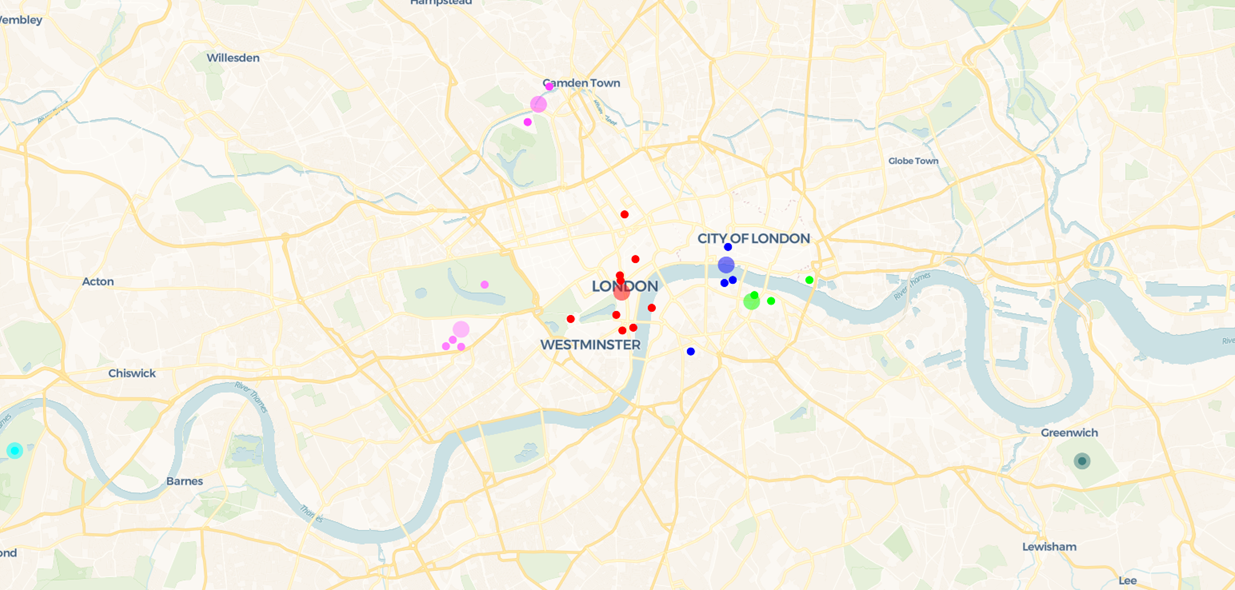
\includegraphics[width = \textwidth]{KMeans_London_Step3}
    \caption{Step3}
\end{figure}
\begin{figure}[H]
    \ContinuedFloat
    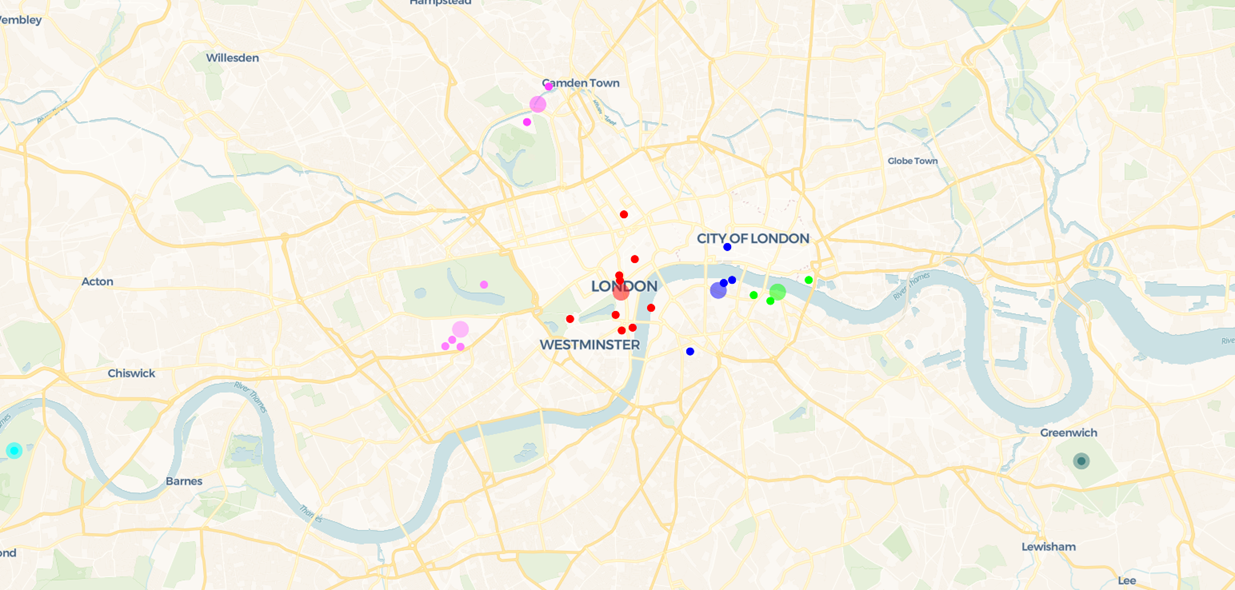
\includegraphics[width = \textwidth]{KMeans_London_Step4}
    \caption{Step4}
\end{figure}

\todo{Short paragraph about how kmeans doesn't intentionally optimise for variance between days.}

\subsubsection{Genetic Clustering}
\todo{Explain genetic clustering}
\subsubsection{Genetic Centroid-based Clustering}
\todo{Explain genetic centroid-based clustering and how it differs from general clustering.}

\subsection{Routing}\label{subsec:routing}
\todo{Explain purpose of routing/goal of algorithms.}
\subsubsection{Brute Force}\label{subsubsec:brute-force-routing}
\todo{Write brute force explanation}
The brute force algorithm is an exhaustive algorithm that tries every possible route to find one with the least cost.
By checking every route it is guaranteed to find the optimal route, however, its computational cost becomes
impractical as input size grows, having a time complexity of $O(n!)$.\todo{Maybe cite time complexity of brute force?}
Considering we will be comparing algorithms based on their speed and the quality of their results, brute force is a
useful benchmark, providing a lower bound for speed and an upper bound for quality.\\
\\
In our brute force implementation, where n is the number of locations in the route, we will be generating all $n-1!$
permutations of the set $\{1, 2, \mathellipsis, n-1\}$, with each permutation representing the order of locations
visited in a route.
Each route will be evaluated according to our optimisation function, and the route with the lowest cost will be
returned.
We only need to consider $n-1!$ permutations because all our routes will start and end at the same location.\\


\subsubsection{Greedy Routing}\label{subsubsec:greedy-routing}
\todo{Explain greedy routing algorithm}
Greedy routing
\subsubsection{Gift Wrapping}\label{subsubsec:gift-wrapping}
\todo{Explain gift wrapping algorithm}
\todo{Something like: "Once gift wrapping has found a convex hull, a greedy insertion algorithm is used to find the optimal route within the convex hull."}
\subsubsection{Genetic Routing}
\todo{Explain genetic routing}

\subsection{Route Insertion}\label{subsec:route-insertion}
\todo{Explain route insertion, how it is used in route planning and the goal of our algorithms.}
\subsubsection{Brute Force}\label{subsubsec:brute-force-route-insertion}
\todo{Explain how brute force algorithm can be modified for route insertion.}
\subsubsection{Greedy Insertion}\label{subsubsec:greedy-insertion}
\todo{Explain how greedy algorithm can be modified for route insertion.}

\subsection{Trip Generation}\label{subsec:trip-generation}
\todo{Explain trip generation, how it is used in route planning and the goal of our algorithms.}
\subsubsection{Brute Force}\label{subsubsec:brute-force-trip-generation}
\todo{Explain how brute force algorithm can be modified for trip generation.}
\subsubsection{Genetic Trip Generation}
\todo{Explain genetic trip generation}